\chapter{Analyse}

\section{Infrastruktur}


\subsection{Netzwerk}
heterogene Netze machen Probleme - Globale Netze haben Latenz, Paketverlust, usw.; müssen Anforderungen gerecht werden.

\subsubsection{Übertragungsmedium}
Als Übertragungsmedien können neben der klassischen Kabelverbindung auch andere (instabile) Kanäle wie Mobilfunk oder Satelliten in Frage kommen. Um die Kommunikation über alle Medien sicher und zuverlässig zu gestalten, müssen auf technischer Ebene Protokolle genutzt werden, welche es ermöglichen die gegebenen Schutzziele zu realisieren und die Integrität der Daten bei der Übertragung über große Entfernungen zu gewährleisten.

TODO - Übertragungsdistanz - Latenz - Jitter - usw.

\subsubsection{Probleme bei Migration alter Systeme}
Inkompatibilität - spezielle bzw. proprietäre Protokolle - besondere Anforderungen der Shop-Floor-Ebene - Industrial Ethernet


\subsection{Integrationsansätze}

\subsubsection{Konsolidierung der Netzwerkkommunikation}
TODO - alles spricht OPC UA

Ansatz: Teuer, aufwendig, nicht möglich, da embedded System bzw. keine Ressourcen oder keine Schnittstellen

\subsubsection{Gatewaykommunikation}
TODO - siehe Trumpf, axoom -> Gateways übersetzen von heterogener Netzwerkkommunikation in Protokollstandard für unternehmensübergreifende bzw. externe Kommunikation.

Ansatz: Softwareschwachstellen, Softwarefehler, müssen viele Herstellerprotokolle unterstützen - Probleme? - bekommt man Appliance?

\section{Protokollanalyse}
\subsection{OPC UA}
\subsection{DDS}
\subsection{MQTT}
\subsection{CoAP}

\section{Angriffsvektoren}
\subsection{Verschlüsselung}
\subsection{Paketversand}
\subsection{TODO}

\section{Maßnahmenkatalog}
\subsubsection{Defense in Depth Strategie - TODO (Kuipers,2006)}
TODO - Beschreibung und Einordnung der Defense in Depth Strategie

\begin{figure}[h]
    \centering
    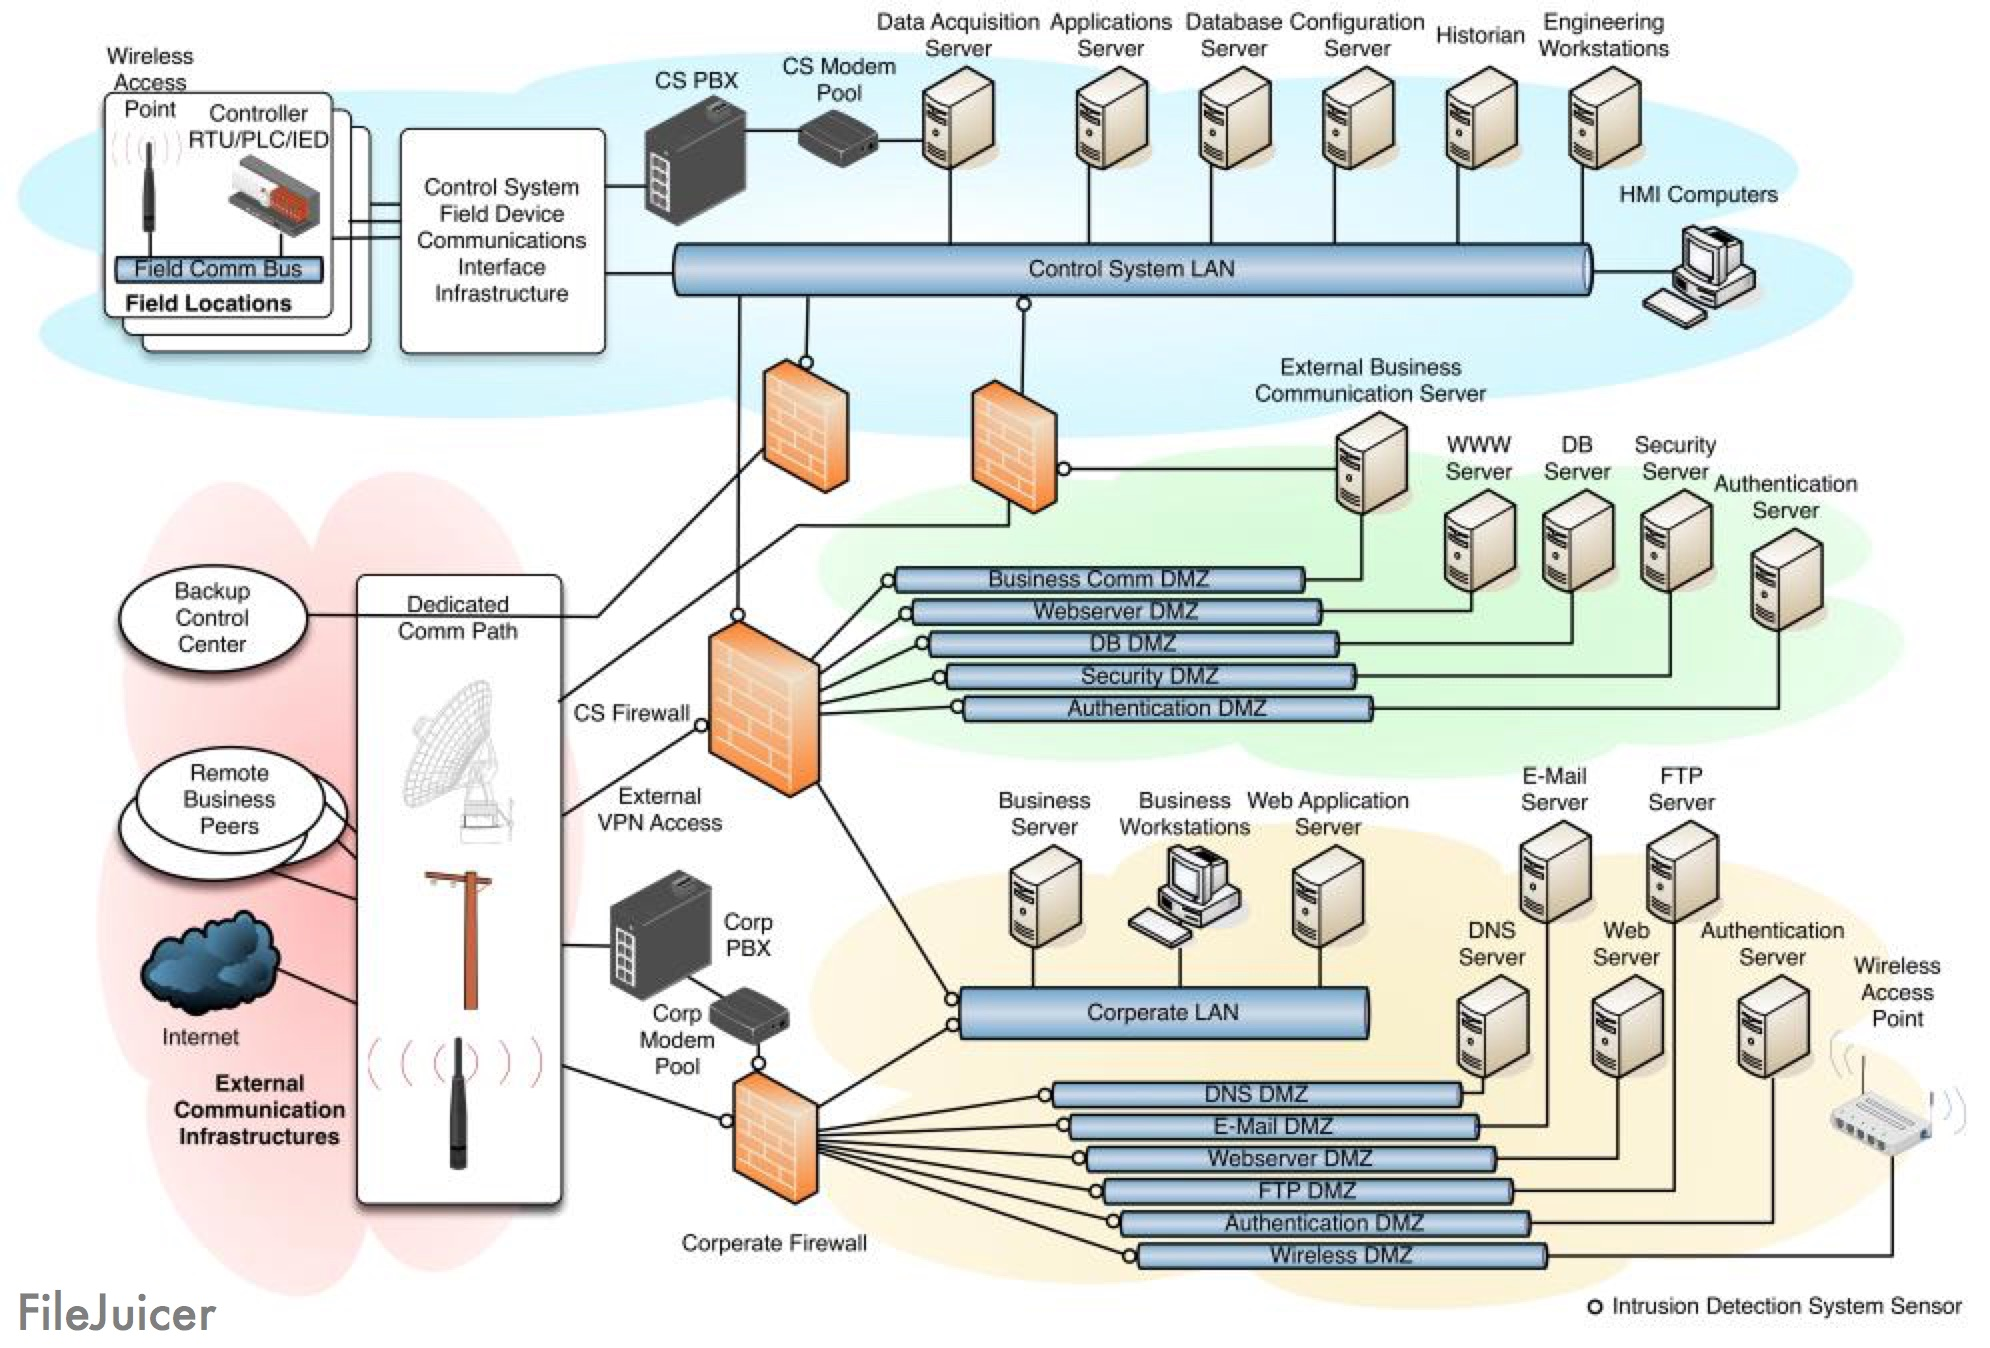
\includegraphics[width=15cm]{defense-in-depth-strategie}
    \caption{Defense in Depth Strategie - TODO ref. Kuipers,2006}
    \label{Kap3:Defense-in-Depth}
\end{figure}

\subsection{TODO}

\section{Auswertung der Ergebnisse}
TODO - Grundlage der Implementierung!